%% Elsevier CAS double-column manuscript, prepared from the
%% els-cas-templates bundle (cas-dc.cls, version 2.4).
%% Body, numbers, tables, figures and citations are the same as the
%% Word manuscript. Author details can be completed from the author profile.

\documentclass[a4paper,fleqn]{cas-dc}

\usepackage[numbers,sort&compress]{natbib}
\usepackage{siunitx}
\usepackage{verbatim}
\usepackage{xurl}
\Urlmuskip=0mu plus 1mu\relax
\def\UrlBreaks{\do\/\do\-\do.\do\=\do\?}

%% Supplementary tables: numbered S1 and S2 in the supplementary document.
\newcommand{\tabS}[1]{Table~S#1}

\begin{document}
\let\WriteBookmarks\relax
\def\floatpagepagefraction{1}
\def\textpagefraction{.001}

\shorttitle{Historical review under finite monitoring retention}
\shortauthors{J.~Zhang}

\title[mode = title]{Historical review under finite monitoring retention: Complete compression, semantic summaries and service boundaries}

%\tnotemark[1]
%\tnotetext[1]{Corresponding author.}

%% Author block: complete the name, affiliation and e-mail from the author
%% profile before submission. The template fields are left active so the
%% compile below satisfies the class requirements.
\author[1]{Junjie Zhang}
\cormark[1]
\ead{junjiezhang2024@shisu.edu.cn}
\credit{Conceptualization, Methodology, Software, Formal analysis, Investigation, Data curation, Writing -- original draft, Writing -- review and editing, Visualization}

\affiliation[1]{organization={Shanghai Academy of Global Governance \& Area Studies, Shanghai International Studies University},
                city={Shanghai},
                postcode={201620},
                country={China}}

\cortext[cor1]{Corresponding author}

\begin{abstract}
Historical review of monitoring outputs asks for the first threshold crossing, its logged value, or every high record in an interval, often after the stream has been compressed or expired. We compare six retention designs on these two review tasks under one 16 byte record contract and identical byte budgets, using 116 histories from 28 servers and two spacecraft missions. Complete compression preserves 57 of 60 coarse histories within 256 KiB and all 60 within 1 MiB, while denser streams leave 53 of 56 within 256 KiB. The Full if fits strategy, which keeps complete history when it fits and otherwise stores complete group summaries with deterministic filling, reconstructs 2,247 first records and 2,174 complete reports from 2,329 positive queries, against 2,167 and 2,167 for complete storage alone. As queries age under chronological retention, coverage summaries recover 56 of 134 first records on the constrained fine server, compared with 24 of 134 for an adaptive policy that favors recency; forecasts based only on past growth produce false feasible and false infeasible capacity decisions, so designers can choose complete compression, narrower exact review, or explicit unavailability from task, age, and encoded size.
\end{abstract}

\begin{highlights}
\item A 16 byte record contract and actual byte accounting make six retention designs directly comparable.
\item Complete compression fits 57 of 60 coarse histories at 256 KiB and all 60 at 1 MiB.
\item Complete group summaries and residual filling change which review tasks remain answerable.
\item Chronological expiration reverses the static ranking on the constrained fine server.
\item A measured decision procedure separates complete, narrower exact, and unavailable history.
\end{highlights}

\begin{keywords}
anomaly monitoring \sep historical review \sep finite retention \sep query completeness \sep time series \sep compressed storage
\end{keywords}

\maketitle

\section{Introduction}\label{sec:intro}

Historical review begins with a concrete question about a past decision. A reviewer may ask when a channel first crossed its recorded threshold, which value was logged at that decision, or whether every high score in a later interval remains available. Grafana exposes alert state history with state changes, their times, and evaluated values, including periods when notifications were muted \cite{Grafana2026State}. Alertmanager groups, deduplicates, and inhibits notifications before delivery \cite{Prom2026Alertmanager}. These interfaces show that historical inspection belongs to monitoring practice. They also show that notification delivery and evidence retention are separate functions. A quieter notification stream can coexist with an archive that has lost the records needed for a later query.

Finite retention turns that separation into a design choice. Prometheus supports compressed local storage, configurable time and size retention, and remote storage \cite{Prom2026Storage}. Loki exposes configurable log retention \cite{Grafana2026Loki}. Compression often makes complete monitoring history affordable. A lossy summary becomes useful when it supports a narrower service at a lower byte cost, or when it extends the age range over which some answer remains possible. The two services answer different questions. A retained high score proves that a crossing occurred, while the identity and value of the first crossing are separate facts. A support map can locate the first high while leaving its logged value unavailable. An empty sample may mean that the interval was negative or that the interval was omitted. Once these distinctions enter the design, retention quality depends on the question being answered.

Research on incomplete information supplies the logical standard for those answers. Completeness statements can certify that a query result is complete even when the full database is unavailable \cite{RazniewskiNutt2011}. Certain answer semantics define the information on which every compatible database agrees \cite{Libkin2015}. Both ideas apply directly to a monitoring archive. A complete bucket can exclude unrecorded highs, and a retained witness can establish existence without establishing precedence. The missing element is the resource consequence. The same completeness logic can be implemented with a support bitmap, a complete group summary, or a full numerical archive, and these representations consume different bytes and answer different tasks. Monitoring research has concentrated on detection quality, alarm forecasting, and computational cost \cite{Strem2025APT,Mejri2024Evaluation}. Compression research has concentrated on encoding size, error bounds, and query support \cite{Jugel2014M4,Jensen2018ModelarDB,Tang2025IoTDB}. What remains open is a task level comparison of what each retained representation can answer under one budget and one retention timeline.

We address that question with two executable tasks. Trigger reconstruction returns yes, no, or unknown for a channel and index set. On a positive scope it returns the first high record with its original score, last value of the completed window, and review context. Report reconstruction returns every requested high record with a separate completeness flag. Both tasks are checked against the full original record. We hold fitted PCA and ridge scores fixed across 28 SMD devices and two ESA missions. We add paired fine cadence SMD streams from the same fitted models and compare six representations at 64 and 256 KiB. Every format carries the same 16 byte atom, schema, provenance, usability map, and index metadata. A chronological replay then closes 1,024 decision chunks, evicts old history under a common cap, and queries the surviving snapshots at ages up to the full observed prefix. A separate forecast exercise asks whether past byte growth can set the next quarter's capacity.

Three findings frame the study. Complete compression is often sufficient: it fits 57 of 60 coarse histories at 256 KiB and all 60 at 1 MiB, and 53 of 56 fine SMD histories at 256 KiB. Strong summaries change the ranking at the margin. On 2,329 positive fine SMD queries at 256 KiB, complete storage alone reconstructs 2,167 first records and 2,167 complete reports; the Full if fits strategy reaches 2,247 and 2,174. Age changes the ranking again. On the constrained fine server, coverage summaries recover 56 of 134 first records, complete FIFO recovers 24, and the adaptive policy recovers 24; the adaptive policy retains only three chunks at the final snapshot, so its static advantage disappears under chronological admission.

The contribution is a controlled, task level account of how retention design changes review service. The new element is the joint treatment of two different review outputs, actual serialized bytes for every format, and chronological expiration on the same histories. It links an established completeness standard to these measurements. It shows where a complete archive is the simplest sufficient design, where a semantically complete summary recovers tasks beyond an archive that stores only support, and where expiration makes the requested history unavailable regardless of representation. The practical output is a decision procedure. Compute the actual complete size for the record contract and horizon, then compare it with the capacity and required query age. Choose the representation that supplies the needed output and verify encoded bytes at admission. These results give monitoring system designers a defensible basis for choosing among complete compression, narrower exact review, and explicit unavailability.

\section{Related work}\label{sec:related}

\subsection{Monitoring delivery and historical evidence}

Monitoring interfaces define the practical starting point. Grafana alert state history records state changes, their times, and evaluated values, including muted periods \cite{Grafana2026State}. Alertmanager separates grouping, deduplication, and inhibition from long term evidence \cite{Prom2026Alertmanager}. These functions motivate the review tasks but leave the archive design open. Prometheus and Loki expose retention controls and compressed storage \cite{Prom2026Storage,Grafana2026Loki}, so an operator can choose how much history to keep. The choice is usually expressed as time or bytes, while the review question is expressed as a record and an interval. Our comparison makes that translation explicit.

Monitoring research has pursued different objectives. Alarm prediction anticipates future events from current telemetry \cite{Strem2025APT}. Anomaly detection benchmarks compare detector accuracy and deployment cost across methods \cite{Mejri2024Evaluation}. Both are upstream of the archive. They determine which scores and alerts exist, while historical review determines which of those outputs remain recoverable. A more accurate detector leaves an archive that dropped the first high record unchanged, and a larger archive leaves detection unchanged. This separation is why we hold the score generators fixed and evaluate the archive as an independent system component.

\subsection{Completeness and the semantics of an answer}

Completeness theory provides the correctness standard. Razniewski and Nutt distinguish local completeness from query completeness and characterize when completeness statements entail a complete answer \cite{RazniewskiNutt2011}. A complete bucket statement can certify that no high was omitted from a range; a retained witness can certify existence at a point. The two facts support different conclusions. Libkin shows that certain answers depend on the query and on the representation of incompleteness, and that a single intersection of answer tuples can be misleading \cite{Libkin2015}. We therefore type the answer: yes, no, or unknown for support; a first position with its original atom for trigger reconstruction; a complete or partial list for report reconstruction. Certification requires agreement across all histories compatible with the retained bytes, including group counts, roles, and usability. This application of established semantics gives the archive a precise contract that can be tested against a reference.

\subsection{Summaries, compressed history and bounded retention}

Visualization synopses and time series compression provide the nearest implementation alternatives. M4 selects first, last, minimum, and maximum records for time groups and preserves a line rasterization property under stated conditions \cite{Jugel2014M4}. Its database keeps the original history and recomputes groups for a new interval, so the synopsis is a view rather than a permanent substitute. MinMaxLTTB reduces a series for rendering while preserving visual shape \cite{VanDerDonckt2023}. These methods optimize what a chart shows. A permanent archive must answer record level queries after the source is gone, which is a different objective.

Queryable compression already combines representation choice, fallback, and access. ModelarDB selects models online, distinguishes temporary and finalized segments, and supports lossy or lossless storage with uncompressed fallback \cite{Jensen2018ModelarDB}. Gorilla and Chimp exploit XOR and leading zero structure for reversible floating point compression \cite{Pelkonen2015Gorilla,Liakos2022Chimp}. Serf adds streaming compression with numerical error bounds \cite{Li2025Serf}. CompressIoTDB supports operations on compressed representations and selective decompression \cite{Tang2025IoTDB}. These systems establish complete compression as a serious comparator and show that a buffer, an index, or a fallback is an engineering option with a measurable cost. Our comparison holds these engines fixed as external references. It holds the record contract fixed and asks which review outputs survive at a given encoded size.

The remaining question is task level. A support map spends bytes on exact presence and absence before it spends bytes on values. A complete group summary spends bytes on counts and roles, and those roles can certify earlier negatives without a bitmap. Residual capacity can then add original atoms without changing either contract. The three designs can therefore answer different subsets of the same workload at the same budget. The studies above evaluate compression ratio, error, or query latency. They leave open the joint first record and complete report service under a common budget and a common expiration policy. That comparison is the empirical contribution of this study.

\section{Materials and methods}\label{sec:methods}

\subsection{Data and score streams}

The coarse streams contain 60 frozen seed zero fits: PCA and ridge for 28 Server Machine Dataset (SMD) devices and two ESA Anomaly Detection Benchmark missions. SMD has 38 variables per device and 327 contiguous binary label incidents \cite{Su2019Omni}. Its published interpretation labels are matched to these intervals before any archive outcome is examined. Zero based, half open intervals match 322 incidents exactly, three partially, and two not at all. The exact cohort supplies 2,254 event dimension pairs. A conservative sensitivity excludes one ambiguous event, leaving 321 incidents and 2,251 targets. The 322 incident cohort is an annotation subset of the 327 source incidents. Contribution dimensions describe annotated participation rather than physical causal roots.

The 708,420 SMD test rows agree with the official values after float32 conversion. The cached binary labels agree exactly. Windows of ten samples produce 70,828 complete coarse decisions, with 140 trailing rows unable to form a complete window. SMD reports a nominal one minute sampling interval \cite{Su2019Omni}, which supplies a scale for localization error rather than an operator work schedule. ESA contributes 58 channels and 55 event identities in Mission 1, and 47 channels and six event identities in Mission 2 \cite{DeCanio2025ESA,Kotowski2026ESA}. Its released timestamps have an anonymizing affine transformation. Unknown annotation regions are excluded from active evaluation scopes.

The score generators use six per channel window features: mean, last, standard deviation, minimum, maximum, and endpoint change. PCA retains 90\% of fitting variance \cite{Jolliffe2016PCA}. Ridge predicts from four preceding coarse windows with regularization 10 \cite{Hoerl1970Ridge}. Let $e_{tj}$ be the mean absolute residual over the six scaled features. Calibration sets
\begin{equation}\label{eq:calib}
\begin{aligned}
q_{tj}&=\frac{e_{tj}}{\max\{Q_{0.95}(e_{\mathrm{cal},j}),10^{-6}\}},\\
\tau&=\max\{Q_{0.995}(\max_j q_{\mathrm{cal},j}),10^{-6}\}.
\end{aligned}
\end{equation}

SMD fits the first 80\% of official training rows and calibrates on the final 20\%, before evaluating the official test sequence. ESA fits usable windows before its three month calibration interval. No test event or dimension label enters fitting, threshold calibration, or archive selection.

For the cadence comparison, we use existing SMD score caches at single sample steps for all 56 device and model pairs. They apply the same fitted models, features, scaling, and thresholds as the paired coarse streams. At shared completed window positions, all channel scores and threshold decisions agree exactly. The comparison therefore changes the density of decisions while holding the detector fixed. The original coarse review tape is projected onto source sample time to define the context version. Cached fine ESA analyses are selected around events, contain gaps, and use numerical PCA refits; the primary fine comparison therefore uses SMD, where the paired streams are complete and model identical.

\subsection{Record contract and executable review tasks}

At decision index $t$ and channel $j$, the archived high support is
\begin{equation}\label{eq:support}
h_{tj}=m_t\,\mathbf{1}\{q_{tj}\geq\tau\},
\end{equation}
where $m_t$ denotes input usability and $q_{tj}$ is the frozen score. A high atom contains decision index (uint32), channel (uint16), arrived review context version (uint16), score (float32), and unscaled last value of the completed window (float32), totaling 16 bytes. The last value can be a preprocessed counter increment. The contract excludes below threshold scores, full windows, native waveforms, and any change to the original rule. A header records the schema, channel identities, threshold, regular clock, and source provenance. A separately compressed decision usability bitmap is charged to every format, so an unusable input is distinguishable from a usable decision with no high. The bitmap is shared across channels because usability is shared in these streams.

Trigger reconstruction takes a rule, channel, and finite index set $I$ and returns yes, no, or unknown for $H(j,I)=\{t\in I:h_{tj}=1\}$. On a positive scope it returns the atom at $\min H(j,I)$ with a certificate of the first position. Primary success requires the certified first position, its original numerical atom, and a precedence certificate that establishes the position. Empty scopes return no with an empty report. A nonempty negative scope requires evidence that no high is compatible with the retained state.

Report reconstruction returns all retained requested high atoms and a separate flag that states whether the report is complete. A partial report remains useful as partial information and carries a completeness flag set to false. The two tasks make the consequence of information loss testable: an original model output report is either reconstructed or returned as unavailable. They characterize archive outputs and leave analyst behavior, time saved, physical failure detection, and fault resolution outside the measured scope.

Exact recovery is the declared replay audit service. A secondary empirical endpoint accepts an original retained atom within one decision of the reference first, with absolute differences in score and last value at most 0.01 in their stored coordinates and an identical context version. The tolerance is evaluated against the complete reference. It is an empirical fidelity endpoint, separate from a certificate for a retained value. The exact service remains the primary comparison.

Notification delivery is held fixed. Parent deduplication for delivery and the earlier locking rule have identical notification times on the same realized tape, so archive representations receive no notification reduction credit. The upstream review tape is simulated selective perfect oracle feedback. An archived context version counts reviews that have already arrived and leaves the frozen baseline score unchanged. The online archive receives neither future review arrivals nor final history information.

\subsection{Completeness semantics and certification}

Let $\Omega(A)$ be the histories compatible with the retained bytes of archive $A$, including its admitted ranges, exact support, usability, summary roles, group counts, and numerical atoms. An output is certified only when all compatible histories give that same typed output. This applies established completeness and certain answer ideas \cite{RazniewskiNutt2011,Libkin2015}. Missing bytes and omitted groups impose no unrecorded completeness assumption.

For ordinary range coverage, a retained positive at $f$ can certify first if every queried index strictly before $f$ is known negative. The position $f$ can lie outside a separate negative coverage container. For example, known negatives at 1 and 2 plus a retained positive at 3 certify first equal to 3 on $I=\{1,2,3\}$. Strong summaries supply further deductions. A complete group for a time bucket and channel records its boundaries, high count, and the first, last, minimum score, and maximum score roles. A first high at 20 in a complete bucket covering 0 to 99 certifies no high on 0 to 19 and first equal to 20 on 0 to 30 without a bitmap. Empty groups are explicitly represented and billed. Only an admitted group carries negative evidence.

The decoder propagates forced positive and negative positions from these facts. In each disjoint complete group $g$, let $U_g$ be the still undetermined positions and $r_g$ its remaining required positives after known positives are removed. For query $I$, write $u_g=|I\cap U_g|$ and $n_g=|U_g|$. If $p$ positives in $I$ are already known, and $v$ queried positions remain wholly unconstrained, the compatible high count bounds are
\begin{equation}\label{eq:bounds}
\begin{aligned}
L&=p+\sum_g\max\{0,r_g-(n_g-u_g)\},\\
U&=p+v+\sum_g\min\{r_g,u_g\}.
\end{aligned}
\end{equation}

Yes is certified when $L>0$, and no when $U=0$. First is certified when $L>0$ and the earliest and latest compatible first positions coincide. A complete numerical report requires that the retained original atoms exhaust the compatible high positions: $L=U=N_{\mathrm{returned}}$. Unretained float32 last values of the completed windows remain unrestricted, even when score extrema constrain a possible score. Support information alone identifies positions; a missing original atom remains unavailable even when support is complete.

Finite memory has an elementary worst case limit. With one channel always high, a single notification parent can accompany $2^{(C-1)T}$ arbitrary histories on the remaining channels. Exact singleton support answers require at least $(C-1)T$ bits in the unrestricted case, because distinguishable histories need distinguishable retained states. Exact numerical recovery adds further states. This bound defines the point at which a finite archive must narrow its supported history or task.

\subsection{Strong representations and actual byte budgets}

All comparisons use the same record semantics and count actual serialized bytes. \textbf{Complete} selects the smaller of separately zlib compressed numerical columns and a compressed support bitmap plus numerical columns ordered by channel. Both decode all original high atoms. An oversized complete candidate is explicitly declined. Its required bytes and the small refusal frame are reported separately, so the frame is charged as a failed archive.

\textbf{Bitmap+change} preserves full high support and the original parent and channel change witnesses: first, last, minimum score, maximum score, and changes of at least $0.25\tau$ from the preceding selected witness. Parent groups are reconstructed from consecutive highs from any channel. Numerical witnesses are admitted chronologically if needed. \textbf{Bitmap+change+fill} first uses the identical base selection, then fills the remaining 16 byte slots with additional original atoms chosen uniformly by deterministic time rank. It adds records according to a fixed time rank and ignores labeled query outcomes.

\textbf{Coverage summary} stores complete fixed time buckets for each channel, their high counts, and first, last, minimum score, and maximum score roles, with deduplicated original atoms for those roles. The initial width is 256 decisions. In the retrospective fixed horizon comparison it doubles the width until the complete candidate fits. If a whole history bucket exceeds capacity, only wholly admitted groups confer completeness. \textbf{Coverage+fill} uses the same base groups and spends remaining bytes on the same deterministic time rank rule. \textbf{Full if fits} first tests the actual complete candidate. If it fits, complete history is retained; otherwise the coverage+fill service is used. The static comparison is an offline reference at the finished target horizon.

Every format charges its JSON schema and provenance, binary framing, usability map for inputs, group records, support map, and numerical payload. Group metadata are compressed, and numerical fill records remain raw 16 byte atoms. Method identifiers have equal fixed lengths, which prevents naming overhead from changing which final slot fits. The test capacities are 64 and 256 KiB. They are experimental conditions rather than measured deployment requirements. For every history we also report
\begin{equation}\label{eq:rho}
\rho=\frac{B}{C_{\mathrm{complete}}},
\end{equation}
where $C_{\mathrm{complete}}$ is the actual complete compressed size under the same record and metadata contract. This ratio separates a regime in which complete storage is feasible from tradeoffs that depend on resources without shrinking capacities or duplicating data to create a bottleneck. Actual bytes, slack, and unsaved candidate atoms accompany every task outcome.

\subsection{Workloads, online retention and evaluation}

Static annotated queries use the full known active interval on each SMD matched contribution dimension or ESA affected channel. Disjoint spans remain index unions. Labels define evaluation scopes after representation construction and remain outside storage decisions. The labeled denominator includes empty scopes and targets with no high. Positive task rates condition explicitly on emitted evidence. A workload independent of labels adds 16 evenly distributed starts at lengths 1, 10, 100, and 1{,}000 decisions with deterministic rotating channels, plus two empty queries. These are declared software workloads rather than estimates of analyst behavior.

The unified online comparison uses four streams: Mission 1 PCA, Mission 1 ridge, and the constrained machine 3-4 ridge at coarse and fine cadence. Each receives identical chronological arrivals and closes the same 1{,}024 decision chunks, including empty chunks. Complete, bitmap\allowbreak+change, and coverage summary policies serialize the incoming closed chunk and FIFO expire older chunks to remain within the common global cap. A chunk that is too large on its own is explicitly rejected. The adaptive policy stores a new complete chunk if the current budget allows. Otherwise it expires old chunks until a coverage summary can fit, then fills the remaining capacity with original records from that incoming chunk. This policy is concrete, uses only past data, and favors recent history. Expired source records are unavailable to every policy. Parent groups are split at chunk boundaries in the online comparison. A 256 decision sensitivity on the constrained server tests whether the complete policy's failures are artifacts of oversized chunks.

Queries run at four approximately quarterly closure times. Scheduled queries use lengths 1, 64, 1{,}024, and 4{,}096 decisions, with endpoints at ages of 0, 1, 4, and 16 chunks and at 25\%, 50\%, and 75\% of the observed prefix. Additional endpoints come from eight deterministic quantiles of already observed high decisions, at lengths 64 and 1{,}024. They are generated from arrived model output without incident labels. Age is the distance from the query's final index to the latest observed index and is separate from any observed alert to human response delay. Age, requested length, partial retained range overlap, and intersection with an actually rejected chunk are recorded separately. Rejected chunk intersection comes from the offline admission log; the charged snapshot alone leaves it ambiguous. Overlapping queries and backbones are related observations.

Each snapshot has one charged shared header, an actual binary directory, and the retained chunk payloads. Query execution reopens the saved snapshot and decodes relevant payloads before comparing the returned result with the complete reference. Persistent bytes are bounded after each closure. Queries run at closures, so every answer is served from a persisted snapshot. Open chunk payload and tracked transient payload costs are reported separately as partial memory accounting. Warm cache wall clock query and close p95 include this Python implementation's file access and serialization. The numbers describe the tested access path rather than a production service level guarantee.

A separate fixed rule prefix exercise forecasts the next quarter's complete compressed requirement using only earlier observed byte increments, with an unbuffered rule and a fixed 1.25 payload margin. The all history extension follows a smaller pilot with the same rule and margins. It reports false feasible and false infeasible capacity decisions rather than selecting a successful forecast from held future results. This exercise tests whether a capacity recommendation inferred from the past preserves the next service horizon.

Verification checks all reopened numerical files against source atoms and every certified task answer against the complete reference. An independent possible world oracle enumerates 64 support histories with six positions, seven retained configurations, and all 64 index subsets. It checks false certification and avoidable refusal for support, first position, and complete report availability. Explicit cases include empty queries, nonempty negatives, partial coverage, unusable inputs, known positives outside complete ranges, and absolute time chunk decoding. The online audit adds 16{,}320 query subsets over 96 snapshot conditions. These finite domain checks supplement the rules and support the interpretation of measured losses.

\section{Results}\label{sec:results}

\subsection{Denser decisions increase evidence availability and complete history cost}

Fine decisions change the relevance of the archive task and its resource requirement. All 327 SMD incidents have a completed decision within their active interval at the fine cadence, compared with 249 at the coarse cadence. On annotated variables, the number of incidents producing at least one high increases from 122 to 216 for PCA and from 135 to 224 for ridge. Positive incident dimension targets increase from 749 to 1{,}101 and from 932 to 1{,}228, respectively, out of the same 2{,}254 annotated targets. These are gains in frozen model output availability, separate from anomaly detection. The fine streams still leave 106 and 98 of the 322 exactly annotated incidents without an annotated variable high for PCA and ridge. \tabS{1} of the supplementary information separates the any channel, annotated channel, and observation opportunity denominators.

The cost increase is substantial and uneven. Original high records increase from 24{,}415 to 238{,}339 for PCA and from 111{,}954 to 1{,}124{,}754 for ridge. Median complete compressed size across the 56 server histories increases from 6{,}338 to 39{,}840 bytes, and the largest history increases from 305{,}207 to 2{,}743{,}495 bytes. The denser stream leaves many histories inexpensive. At 256 KiB, complete storage fits 53 of 56 fine histories, including all 28 PCA histories. At 1 MiB, it fits 55 of 56. The earlier finding that 1 MiB sufficed for all coarse histories therefore does not extend to the denser server stream (Table~\ref{tab:1}, Fig.~\ref{fig:1}a).

\begin{table*}
\caption{Complete storage under the same high record and metadata contract. Histories are device and model or mission and model combinations and are related observations. KiB denotes 1{,}024 bytes. The 1 MiB column is a feasibility census of actual complete sizes.}
\label{tab:1}
\small
\begin{tabular*}{\textwidth}{@{\extracolsep{\fill}}lrrrrl@{}}
\toprule
Source and cadence & Histories & Fit 64 KiB & Fit 256 KiB & Fit 1 MiB & Median / maximum bytes \\
\midrule
ESA, coarse & 4 & 1 & 2 & 4 & 210{,}967 / 554{,}282 \\
SMD, coarse & 56 & 54 & 55 & 56 & 6{,}338 / 305{,}207 \\
SMD, fine & 56 & 36 & 53 & 55 & 39{,}840 / 2{,}743{,}495 \\
\bottomrule
\end{tabular*}
\end{table*}

ESA remains an upstream boundary. Its 61 anomaly identities yield affected channel evidence for only eight PCA and nine ridge event identities in the coarse streams. Archive success conditional on a positive target measures service coverage rather than event detection. The spacecraft histories also show that high record density and compressibility depend on the model: only two of the four complete histories fit 256 KiB. These results argue for measuring complete cost for the actual rule, cadence, and horizon before adopting lossy retention.

\subsection{Strong summaries and slack filling change the available task service}

The primary static comparison evaluates 116 related histories: the 60 original coarse fits and 56 paired fine streams. Every method uses the same records and query scopes within a history. Table~\ref{tab:2} and Fig.~\ref{fig:1}b show fine SMD at 256 KiB, where 2{,}329 of the 4{,}508 annotated model specific scopes contain high evidence. Complete storage supplies 2{,}167 joint first reconstructions and 2{,}167 complete positive reports. Its missing results are concentrated in the three declined ridge histories. Full if fits supplies 2{,}247 joint first reconstructions and 2{,}174 complete reports, with seven unknown support answers across all 4{,}508 queries. Its gain over complete storage is 80 positive first reconstructions and seven complete reports.

\begin{table*}
\caption{Fine SMD task service at 256 KiB. Joint first and complete report use the 2{,}329 positive annotated queries. Certified negative and unknown use the full 4{,}508 query workload, which contains 2{,}179 reference negative queries. All method answers are checked against the same full reference. Complete denotes an archive that stores full history or declines service; its small refusal frame is charged separately from successful compression.}
\label{tab:2}
\small
\begin{tabular*}{\textwidth}{@{\extracolsep{\fill}}lrrrr@{}}
\toprule
Representation & Joint first & Complete positive report & Certified negative & Unknown support \\
\midrule
Complete & 2{,}167 & 2{,}167 & 2{,}174 & 167 \\
Bitmap + change & 2{,}180 & 633 & 2{,}179 & 0 \\
Bitmap + change + fill & 2{,}199 & 1{,}521 & 2{,}179 & 0 \\
Coverage summary & 1{,}912 & 325 & 2{,}161 & 79 \\
Coverage + fill & 2{,}123 & 1{,}462 & 2{,}165 & 29 \\
Full if fits & 2{,}247 & 2{,}174 & 2{,}179 & 7 \\
\bottomrule
\end{tabular*}
\end{table*}

Complete group semantics make summaries competitive rather than isolated witnesses. At 64 KiB, coverage summaries reconstruct 1{,}904 first records, compared with 1{,}777 for bitmap+change and 1{,}244 for complete storage. At 256 KiB, the ordering reverses between the two summaries: bitmap+change reconstructs 2{,}180 first records and coverage summary 1{,}912. Full support protects arbitrary subinterval precedence, while local roles spend fewer bytes on selected original atoms and provide narrower coverage. Each representation wins at one budget. \tabS{2} separates the two backbones and both capacities.

Filling exposes a second distinction. At 256 KiB, bitmap\allowbreak+change\allowbreak+fill increases joint first reconstruction by 19 and complete positive reports by 888 relative to bitmap\allowbreak+change. Coverage+fill increases the corresponding counts by 211 and 1{,}137. Additional records can complete reports even when the base representation already retains their first record; they can also remove support uncertainty by adding positive witnesses. The filling rule is independent of labels, so these gains describe the value of generic residual capacity rather than an optimal allocation. Bitmap filling still leaves 808 positive reports incomplete.

Pooled counts conceal heterogeneity. For ridge at 256 KiB, the device mean joint first rate is 0.889 for complete storage, 0.933 for bitmap+change+fill, and 0.944 for Full if fits, calculated over the 27 devices with positive annotated scopes. Their device minima are 0, 0.368, and 0.467. Full if fits supplies all positive PCA tasks because every fine PCA history fits, yet its worst ridge device still has no complete positive report. These device summaries are descriptive. The two backbones and their overlapping event queries are related observations.

\begin{figure*}
\centering
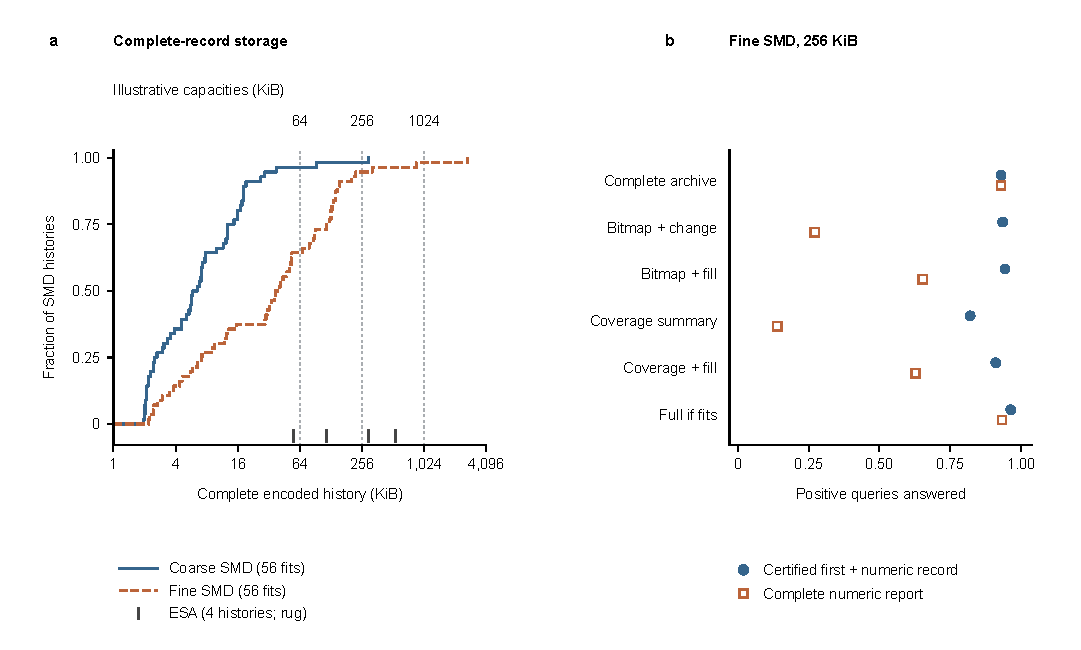
\includegraphics[width=\textwidth]{figs/figure1_storage_task.pdf}
\caption{Complete history cost and finite archive task service. (a) Empirical cumulative complete compressed cost for 56 SMD histories at each cadence, with the four coarse ESA histories shown separately. Vertical guides mark 64 KiB, 256 KiB, and 1 MiB; crossing a guide determines complete storage feasibility under the declared contract. The paired cadence curves reuse fitted models. (b) Joint first reconstruction and complete positive report rates for the six representations on fine SMD at 256 KiB, with 2{,}329 positive annotated model specific queries. The two outcomes require different retained information. They are workload fractions for the declared queries.}
\label{fig:1}
\end{figure*}

\subsection{A constrained history separates spare capacity from irrecoverable task detail}

The constrained coarse server history has a complete archive of 305{,}207 bytes, giving relative capacity 0.859 at 256 KiB. Bitmap+change uses only 78{,}661 bytes and leaves 183{,}483 bytes unused (Table~\ref{tab:3}). Filling increases retained atoms from 4{,}758 to 16{,}225 and joint first reconstruction from 13 of 20 to 14 of 20. It leaves the two complete positive reports unchanged. Most of the available slack can therefore be spent without recovering a whole requested report, while at least one prior first record loss was avoidable under a straightforward fill independent of labels. Both observations matter when interpreting the apparent capacity limit.

\begin{table*}
\caption{Actual bytes and positive tasks on the constrained coarse ridge history at 256 KiB. There are 60{,}483 source atoms and 20 positive annotated targets. Unsaved is the number of original atoms omitted. The complete candidate is declined; its frame uses 1{,}990 bytes while its required complete size is 305{,}207 bytes. Full if fits selects the same state as coverage+fill here and is omitted as a duplicate row.}
\label{tab:3}
\small
\begin{tabular*}{\textwidth}{@{\extracolsep{\fill}}lrrrrr@{}}
\toprule
Representation & Actual bytes & Slack bytes & Unsaved atoms & Joint first / 20 & Complete report / 20 \\
\midrule
Complete, declined & 1{,}990 & 260{,}154 & 60{,}483 & 0 & 0 \\
Bitmap + change & 78{,}661 & 183{,}483 & 55{,}725 & 13 & 2 \\
Bitmap + change + fill & 262{,}133 & 11 & 44{,}258 & 14 & 2 \\
Coverage summary & 20{,}907 & 241{,}237 & 59{,}424 & 10 & 2 \\
Coverage + fill & 262{,}139 & 5 & 44{,}347 & 11 & 2 \\
\bottomrule
\end{tabular*}
\end{table*}

A short real incident shows a task change that record counts conceal. On the constrained fine ridge history, incident 2 and annotated variable 10 have three high records at source samples 6{,}013 to 6{,}015. At 64 KiB, bitmap+change occupies 65{,}528 bytes and certifies the first position, but returns none of the three numerical atoms. The complete group summary occupies 49{,}766 bytes and reconstructs the first atom, including score 215.59866333007812, last value of the completed window 1, and context version 6. It returns only one of the three records, so the completeness flag remains false. Coverage+fill uses 65{,}526 bytes and still lacks the other two records. The case combines a successful original trigger reconstruction with a failed complete report task on an annotated anomaly.

The secondary fidelity criterion preserves the distinction. At 256 KiB on fine SMD, Full if fits has 2{,}259 empirical tolerant first matches, compared with 2{,}247 certified joint successes. Coverage+fill has 2{,}188 tolerant matches against 2{,}123 joint successes. Every tolerant match in this workload already has an exact reference first atom, so the tolerance adds no selected atom beyond exact numerical matching. The difference from joint success concerns the inability to certify precedence from retained information. One coarse decision and one fine decision span different nominal durations, so their tolerance rates are specific to the chosen cadence and tolerances.

\subsection{Online policy rankings depend on how far back the task reaches}

The unified online experiment has 32 stream, capacity, and policy conditions with 5{,}280 queries. All persistent snapshots stay within their charged ceiling. Every evaluated certificate agrees with the reference. Moving the same representations into chronological admission nevertheless changes their service, because resident history competes with incoming complete detail.

On the constrained fine ridge history at 256 KiB, complete FIFO reconstructs 24 of 134 positive first records and 24 complete reports, with 144 unknown support answers among 176 queries (Table~\ref{tab:4}). Coverage summary retains all 24 closed chunks and reconstructs 56 first records and 12 complete reports, with no unknown support on this workload. Bitmap+change reconstructs 50 first records and 12 complete reports, with three unknowns. The adaptive policy, which favors recency, reconstructs 24 first records and six complete reports, with 118 unknowns. Its static Full if fits advantage therefore gives way to a different online ranking. At the final snapshot it retains only three chunks, compared with 21 for bitmap+change and 24 for coverage summary.

\begin{table*}
\caption{Online constrained fine ridge history at 256 KiB with 1{,}024 decision chunks. Positive tasks have denominator 134; support answers have denominator 176. Evictions and p95 timing cover the chronological run. All four policies use identical arrivals and queries. Query timing is warm cache wall clock time for reopening and decoding the archive in this implementation.}
\label{tab:4}
\small
\begin{tabular*}{\textwidth}{@{\extracolsep{\fill}}lrrrrr@{}}
\toprule
Policy & Joint first & Complete positive & Unknown support & Evicted chunks & Query p95, ms \\
\midrule
Complete FIFO & 24 & 24 & 144 & 22 & 10.13 \\
Bitmap + change FIFO & 50 & 12 & 3 & 3 & 4.29 \\
Coverage summary FIFO & 56 & 12 & 0 & 0 & 3.50 \\
Adaptive complete / summary & 24 & 6 & 118 & 21 & 6.63 \\
\bottomrule
\end{tabular*}
\end{table*}

Query age explains a substantial part of that ordering (Fig.~\ref{fig:2}). At an endpoint age no greater than 1\% of the observed prefix, complete FIFO reconstructs 21 of 25 first records and 21 complete reports, compared with 14 of 25 and four for coverage summary. Beyond 25\% of the prefix age, complete FIFO reconstructs none of the 72 positive first records, while coverage summary reconstructs 28. The latter's complete report count over these older scopes is only seven. Retaining older support reconstructs selected first records while leaving some old numerical detail unavailable. These fractions conditioned on age describe declared query scenarios rather than observed analyst delays.

\begin{figure*}
\centering
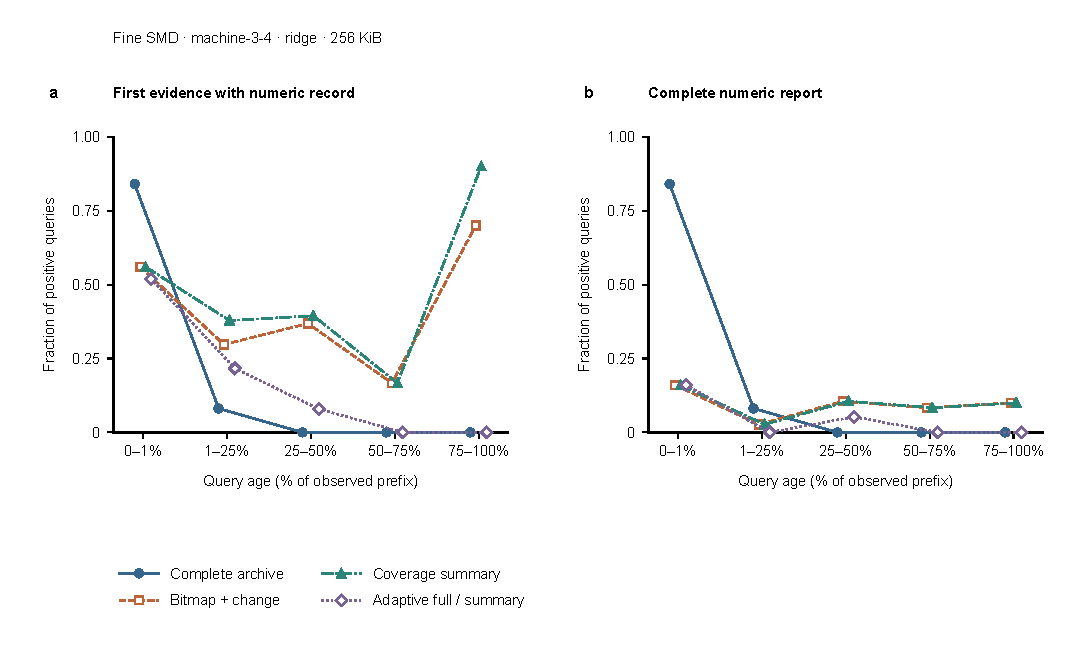
\includegraphics[width=\textwidth]{figs/figure2_online_age.pdf}
\caption{Historical task service changes with query age. Joint first reconstruction and complete positive report rates on the constrained fine ridge history at 256 KiB, for the four chronological policies. Endpoint age is divided by the observed prefix length at query time. The five age groups contain 25, 37, 38, 24, and 10 positive queries. The same queries are used across policies. Complete FIFO favors recent exact detail; the coverage summary preserves more older first records and fewer complete reports. Connecting lines guide comparison between the declared age groups.}
\label{fig:2}
\end{figure*}

The summary advantage depends on the stream. On Mission 1 ridge at 256 KiB, bitmap+change retains all 720 chunks and reconstructs 56 of 69 first records and 48 complete reports with no unknowns. Complete FIFO reconstructs 42 first records and 42 complete reports with 36 unknown answers. Coverage summary reconstructs 38 and 33 with 25 unknowns. On Mission 1 PCA at 64 KiB, complete FIFO instead supplies 22 of 65 joint first reconstructions, exceeding bitmap+change with 17 and coverage summary with 10. Complete group metadata and role records can consume more storage than highly compressible original columns. Representation selection therefore depends on the actual stream rather than on a general preference for summaries.

Smaller chunks reduce rejection while expiration remains. On the constrained fine ridge history at 64 KiB, the 1{,}024 decision complete policy rejects 20 chunks; the 256 decision sensitivity rejects none. In the smaller chunk workload it still has 149 of 176 unknown support answers. At 256 KiB, the smaller chunk complete policy has 115 unknowns, compared with none for coverage summary. The two chunk size runs generate different anchor times and age scenarios, so their task fractions are descriptive comparisons across different query sets. Within each run, all methods share the same queries. Length, retained boundary crossing, and rejected hole results appear in the supplementary information.

Persistent capacity also differs from working memory and access cost. In the constrained fine comparison, the tracked maximum open payload is 522{,}928 bytes, already larger than either persistent ceiling. Tracked transient payloads reach 841{,}448 bytes for complete FIFO at 256 KiB; these partial accounting figures exclude additional Python and codec allocations. At the same capacity, query p95 is 3.50 to 10.13 ms across policies, while block close p95 is 39.22 to 297.48 ms. Mission 1 ridge complete queries reach p95 87.65 ms. These measurements quantify the tested access path.

\subsection{Past cost forecasts support planning within measured error}

The prefix exercise tests 348 next quarter decisions for each capacity and fixed margin. At 64 KiB, unbuffered extrapolation produces 15 false feasible decisions and two false infeasible decisions. A 1.25 payload margin reduces the former to 11 and increases the latter to four. At 256 KiB, both margins leave four false feasible decisions; the larger margin increases false infeasible decisions from one to three. Fine SMD alone contributes 13 of the unbuffered false feasible decisions at 64 KiB. These are errors of a fixed planning rule based only on past data rather than estimates of operational risk.

Bursty compressed growth explains why a fixed margin leaves service exposed. At each forecast origin, Mission 1 ridge grows from 19{,}943 bytes at the first quarter to 274{,}131 bytes at the second. Fine machine 1-1 PCA grows from 8{,}154 bytes at the second quarter to 100{,}580 bytes at the third. The worst census underprediction is 91.7\%, and the buffered rule still underpredicts that requirement by 89.9\%. A low observed complete cost can justify trying complete retention; the next horizon still requires an admission check. Actual admission must verify encoded bytes and expose any scope reduction.

Implementation checks test whether lost service reflects missing information or an unnecessarily conservative decoder. The six position support enumeration checks 28{,}672 query subsets, and the independent multichannel extension checks 32{,}768, including partial group admission, tied nonmonotone scores, and declined files. Both find zero false certificates and zero avoidable unknowns within their stated finite domains. The real static comparison reopens all 1{,}392 budgeted files and reports no false certificate. Actual grid inputs contain no unusable decisions, so unavailable input semantics are exercised by constructed cases. These checks support the interpretation of measured losses without substituting verification counts for application value.

\section{Discussion}\label{sec:discussion}

\subsection{Complete compression is the default when it fits}

Complete compression resolves most histories at the test capacities. It fits all 60 coarse histories at 1 MiB, 57 at 256 KiB, and 53 of 56 fine SMD histories at 256 KiB. A system that can afford the complete encoded history should therefore prefer it. For a history that fits, complete storage supplies every exact output by construction, and no tested alternative can exceed that coverage on the same history. The open question is what happens when the target history exceeds the budget, or when the relevant horizon is longer than the current prefix.

Dense fine decisions create that condition without artificial data duplication or reduced capacities. The constrained server history requires 305{,}207 bytes for a complete archive at 256 KiB, while the fine ridge streams reach 2{,}743{,}495 bytes. These are measured sizes under one record contract. Capacity planning must therefore use the actual rule, cadence, and horizon. A coarse history can fit at 256 KiB while its fine counterpart exceeds the same budget, even when both use the same fitted model.

\subsection{Summary semantics and residual capacity explain the reversals}

Complete group summaries change the ranking because selected records carry information beyond their values. A stored bucket first can establish an earlier negative interval without a support bitmap. A complete count can bound the number of missing highs. The coverage summary uses those facts, so it is a stronger competitor than a point sample with the same number of atoms. At 64 KiB it reconstructs 1{,}904 first records, ahead of bitmap+change with 1{,}777 and complete storage with 1{,}244. At 256 KiB the ordering reverses: full support protects arbitrary subinterval precedence, and bitmap+change reconstructs 2{,}180 first records against 1{,}912 for coverage summary.

Filling explains a second reversal. A base representation can retain the first record of a report while omitting later atoms, so its joint first count understates the value of residual capacity for complete reports. At 256 KiB, bitmap+change+fill adds 19 first reconstructions and 888 complete reports. Coverage+fill adds 211 first reconstructions and 1{,}137 complete reports. The asymmetry is mechanical: a report needs every atom, while a first reconstruction needs one atom and a precedence certificate. The constrained coarse history shows the limit of this remedy. Spending almost all remaining capacity adds one first reconstruction and no complete report, because the missing atoms lie outside the positions that the fill rule recovers.

Chronological admission explains the third reversal. A static archive sees the finished horizon and can choose the best representation for that horizon. An online policy must commit bytes before future queries arrive. Complete FIFO preserves recent detail but expires older chunks; on the constrained fine history it retains 24 of 134 first records. Coverage summary keeps all 24 chunks, so it recovers 56 first records but only 12 complete reports. The adaptive policy prefers incoming complete chunks, retains three chunks at the final snapshot, and recovers 24 first records and six complete reports. Its static advantage comes from complete storage at the finished horizon, a condition that is unavailable to the online policy in advance.

\subsection{A design procedure follows from the measured boundaries}

The results support a short decision procedure. First, compute the actual complete compressed size for the record contract and the longest horizon that must remain reviewable. If that size fits the persistent budget, retain complete history: it supplies both tasks and avoids a semantic fallback. Second, if complete history exceeds the budget, identify the dominant output. A first trigger reconstruction needs exact support around the first high and one original atom; a complete report needs every atom and a completeness certificate. Third, set the required age range. Recent queries favor complete chunks, while older first record queries can favor support preserving summaries. Fourth, verify encoded bytes at admission and return unknown with any partial records when the retained state leaves the requested output undetermined. This procedure uses the measured quantities directly and the declared workload.

The procedure also identifies when a summary is the right engineering choice. A summary is attractive when its semantic roles answer the dominant task at a lower byte cost, or when it extends the age range over which first records remain recoverable. A summary is a poor substitute for complete history when the task requires every numerical atom in a report, because local roles and counts describe selected atoms only. The constrained fine case makes the distinction concrete: coverage summary reconstructs the first atom but returns one of three records, so the first trigger task succeeds while the complete report remains partial.

\subsection{Scope and evidence boundaries}

The conclusions concern declared high score records under the tested retention policies. The study does not measure the frequency of analyst queries, the quality of human decisions, time saved, physical fault detection, or deployment capacity requirements. The 64 and 256 KiB capacities are experimental conditions. A site with inexpensive remote storage and mostly recent queries may have little reason to use a lossy service. A site that needs long support history with sparse exact records faces the tradeoff studied here. These are conditional implications, not observed human benefits.

The recorded outputs impose a ceiling on what any archive can recover. A positive target preservation rate excludes events that never produced a declared high. Fine cadence reduces observation losses, yet both backbones still miss annotated variable evidence for many incidents, and ESA has fewer supported event identities. Neither retention nor complete reports recover an unknown anomaly from absent model output. SMD dimension labels identify annotated contributions rather than physical causal roots. The two ESA missions share benchmark and task structure and are not independent industrial deployments. Their transformed timestamps do not establish operational deadlines.

The 16 byte schema omits full windows and most feature information. An earlier 36 byte richer record check saved all six declared unscaled window features and verified retrieval in 60 files, but those files do not extend the present budget claims. Original fitted predictor objects were not persisted, and fine ESA caches selected around events use numerical refits, so counterfactual score recomputation and bit identical ESA fine replay are unavailable. Saved high score atoms also cannot answer a newly chosen lower threshold or reconstruct below threshold history. These are different record services that require their own storage and validation.

Review updates are simulated selective perfect oracle feedback. Their tags describe arrived context rather than human accuracy, labor, or attention. Prior fine cadence locking lost timely notification identities even while retaining the original score hit identities, and past selected notification policies failed future retention checks. Parent deduplication for delivery has the same notification timestamps as locking on a shared tape. The archive results do not reverse those failures and do not imply notification, safety, or work time gains. Holding delivery fixed makes the archive contribution assessable without assigning it an unmeasured downstream effect.

The implementation checks cover finite domains. The core oracle enumerates 64 support histories with six positions, seven configurations, and all 64 index subsets; the independent extension covers 32,768 multichannel cases; the online audit covers 16,320 query subsets over 96 snapshot conditions. These checks establish correctness within their stated domains and do not enumerate every float32 world or every deployment. The real static comparison reopens 1,392 files with no false certificate. Tracked memory figures are partial lower bounds, and warm cache p95 values describe this Python implementation rather than a production service level guarantee.

\section{Conclusion}\label{sec:conclusion}

Historical review needs a service specification before it needs a compression ratio. The specification has two outputs, a record contract, a byte budget, and a maximum query age. Under that specification, complete compression is the simplest sufficient design whenever the actual encoded history fits. When it exceeds the budget, a complete group summary can recover first records beyond an archive that stores only support, and residual capacity can complete many reports that an archive storing only witnesses leaves partial. Chronological retention can still reverse the ranking, because bytes spent on incoming detail are unavailable for older queries.

The study supplies measured boundaries for those choices. Complete compression fits 57 of 60 coarse histories at 256 KiB and all 60 at 1 MiB, while 53 of 56 fine SMD histories fit 256 KiB. Full if fits reconstructs 2{,}247 first records and 2{,}174 complete reports from 2{,}329 positive queries, against 2{,}167 and 2{,}167 for complete storage alone. On the constrained fine server, coverage summary recovers 56 of 134 first records while the adaptive policy recovers 24. Forecasts based only on past data produce both false feasible and false infeasible decisions. These results give system designers a concrete basis for choosing complete compression, narrower exact review, or explicit unavailability, and they identify the query age and output type at which each choice changes.

\section*{Data and code availability}

ESA Anomaly Dataset version 2 is available under CC BY 3.0 IGO, with credit to the European Space Agency and benchmark contributors, under the terms specific to the IGO. SMD and its interpretation labels are available from the fixed official repository version; the MIT license specific to the dataset was verified separately from the code license. The replication materials document fixed sources and include annotation reconciliation, record and query specifications, execution scripts, serialized archives, results for each history and query, and verification receipts. They are available at \url{https://github.com/williamjay1/historical-review-finite-retention} and archived at \url{https://doi.org/10.5281/zenodo.23646555}. Raw datasets are not redistributed; selected original last values of completed windows occur only within the derived high score service records. The original preparation pipeline and its dependencies on frozen fitted outputs are documented. No human participants were recruited.

\section*{Declaration of generative AI and AI-assisted technologies in the manuscript preparation process}

During the preparation of this work, the author(s) used OpenAI Codex (GPT-5 Codex) for limited Python code assistance and English language polishing; the tool was used on 23 October 2026 and had no access to research data. The author(s) reviewed and edited the output as needed and take full responsibility for the content of the published article.

\section*{Declaration of competing interest}

The authors declare that they have no known competing financial interests or personal relationships that could have appeared to influence the work reported in this paper.

%% Bibliography: numbered, first-appearance order, matching the Word manuscript.
\begin{thebibliography}{20}

\bibitem{Grafana2026State}
Grafana Labs, 2026. View alert state history. Grafana documentation. \url{https://grafana.com/docs/grafana/latest/alerting/monitor-status/view-alert-state-history/} (accessed 9 October 2026).

\bibitem{Prom2026Alertmanager}
Prometheus Authors, 2026. Alertmanager. Prometheus documentation. \url{https://prometheus.io/docs/alerting/latest/alertmanager/} (accessed 9 October 2026).

\bibitem{Prom2026Storage}
Prometheus Authors, 2026. Storage. Prometheus documentation. \url{https://prometheus.io/docs/prometheus/latest/storage/} (accessed 9 October 2026).

\bibitem{Grafana2026Loki}
Grafana Labs, 2026. Log retention. Grafana Loki documentation. \url{https://grafana.com/docs/loki/latest/operations/storage/retention/} (accessed 9 October 2026).

\bibitem{RazniewskiNutt2011}
Razniewski, S., Nutt, W., 2011. Completeness of queries over incomplete databases. Proceedings of the VLDB Endowment 4 (11), 749--760. \url{https://doi.org/10.14778/3402707.3402715}.

\bibitem{Libkin2015}
Libkin, L., 2015. How to define certain answers. Proceedings of the Twenty-Fourth International Joint Conference on Artificial Intelligence, 4282--4288. \url{https://www.ijcai.org/Proceedings/15/Papers/609.pdf}.

\bibitem{Strem2025APT}
Strem, N., Dhami, D.S., Schmidt, B., Kl\"opper, B., Kersting, K., 2025. APT: Alarm Prediction Transformer. Expert Systems with Applications 261, 125521. \url{https://doi.org/10.1016/j.eswa.2024.125521}.

\bibitem{Mejri2024Evaluation}
Mejri, N., Lopez-Fuentes, L., Roy, K., Chernakov, P., Ghorbel, E., Aouada, D., 2024. Unsupervised anomaly detection in time-series: An extensive evaluation and analysis of state-of-the-art methods. Expert Systems with Applications 256, 124922. \url{https://doi.org/10.1016/j.eswa.2024.124922}.

\bibitem{Jugel2014M4}
Jugel, U., Jerzak, Z., Hackenbroich, G., Markl, V., 2014. M4: A Visualization-Oriented Time Series Data Aggregation. Proceedings of the VLDB Endowment 7 (10), 797--808. \url{https://doi.org/10.14778/2732951.2732953}.

\bibitem{Jensen2018ModelarDB}
Jensen, S.K., Pedersen, T.B., Thomsen, C., 2018. ModelarDB: Modular Model-Based Time Series Management with Spark and Cassandra. Proceedings of the VLDB Endowment 11 (11), 1688--1701. \url{https://doi.org/10.14778/3236187.3236215}.

\bibitem{Tang2025IoTDB}
Tang, Y., Zhang, F., Guan, J., Tian, Y., Huang, X., Wang, C., Wang, J., Du, X., 2025. Improving Time Series Data Compression in Apache IoTDB. Proceedings of the VLDB Endowment 18 (10), 3406--3420. \url{https://doi.org/10.14778/3748191.3748204}.

\bibitem{VanDerDonckt2023}
Van Der Donckt, J., Van Der Donckt, J., Rademaker, M., Van Hoecke, S., 2023. MinMaxLTTB: Leveraging MinMax-Preselection to Scale LTTB. 2023 IEEE Visualization and Visual Analytics (VIS), 21--25. \url{https://doi.org/10.1109/VIS54172.2023.00013}.

\bibitem{Pelkonen2015Gorilla}
Pelkonen, T., Franklin, S., Teller, J., Cavallaro, P., Huang, Q., Meza, J., Veeraraghavan, K., 2015. Gorilla: A Fast, Scalable, In-Memory Time Series Database. Proceedings of the VLDB Endowment 8 (12), 1816--1827. \url{https://doi.org/10.14778/2824032.2824078}.

\bibitem{Liakos2022Chimp}
Liakos, P., Papakonstantinopoulou, K., Kotidis, Y., 2022. Chimp: Efficient Lossless Floating Point Compression for Time Series Databases. Proceedings of the VLDB Endowment 15 (11), 3058--3070. \url{https://doi.org/10.14778/3551793.3551852}.

\bibitem{Li2025Serf}
Li, R., Chen, Z., Lu, R., Xu, X., Yang, G., Chen, C., Bao, J., Zheng, Y., 2025. Serf: Streaming Error-Bounded Floating-Point Compression. Proceedings of the ACM on Management of Data 3 (3), 1--27. \url{https://doi.org/10.1145/3725353}.

\bibitem{Su2019Omni}
Su, Y., Zhao, Y., Niu, C., Liu, R., Sun, W., Pei, D., 2019. Robust Anomaly Detection for Multivariate Time Series through Stochastic Recurrent Neural Network. Proceedings of the 25th ACM SIGKDD International Conference on Knowledge Discovery and Data Mining, 2828--2837. \url{https://doi.org/10.1145/3292500.3330672}.

\bibitem{DeCanio2025ESA}
De Canio, G., Kotowski, K., Haskamp, C., 2025. ESA Anomaly Dataset. Version 2. European Space Agency. \url{https://doi.org/10.5281/zenodo.15237121}.

\bibitem{Kotowski2026ESA}
Kotowski, K., Haskamp, C., Andrzejewski, J., Ruszczak, B., Nalepa, J., Lakey, D., Collins, P., Mart\'inez-Heras, J., De Canio, G., 2026. European Space Agency Dataset and Benchmark for Real-World Anomaly Detection in Spacecraft Time Series. Journal of Data-centric Machine Learning Research 3 (23), 1--76. \url{https://data.mlr.press/assets/pdf/v03-23.pdf}.

\bibitem{Jolliffe2016PCA}
Jolliffe, I.T., Cadima, J., 2016. Principal component analysis: A review and recent developments. Philosophical Transactions of the Royal Society A: Mathematical, Physical and Engineering Sciences 374 (2065), 20150202. \url{https://doi.org/10.1098/rsta.2015.0202}.

\bibitem{Hoerl1970Ridge}
Hoerl, A.E., Kennard, R.W., 1970. Ridge Regression: Biased Estimation for Nonorthogonal Problems. Technometrics 12 (1), 55--67. \url{https://doi.org/10.1080/00401706.1970.10488634}.

\end{thebibliography}

\printcredits

\end{document}
